\documentclass[project_eva.tex]{subfiles}
\begin{document}

\subsection*{Interaction}
Eva uses simulation of affectiveness as a clear non-expert way of interacting \cite{Thomaz} . This allows the user to communicate with Eva in a natural way.  This results in a lower learning curve and makes Eva more accessible for the user. Eva signals for interaction by gaining eye-contact with the user. Eva interacts using a combination of lights, sounds and facial movement to cope with potential ailments of old age � such as reduced hearing and vision . For receiving and understanding information from the user, Eva uses keyword-based voice recognition. 

\subsubsection*{Affect Detection}
Eva is able to recognize the level of affection in the words spoken by the user, this is done with speech recognition. Affect detection is necessary for Eva to fully understand what the user is saying, because a message can convey different meanings when loaded with a different emotion.

Detection by words is the simplest form of affect detection that works efficiently, given that the speech recognition module works good enough \cite{affection} . This is done by comparing the recognized words with a list of positively and negatively loaded words, Eva is able to distinguish positive and negative feedback.
 
\subsubsection*{Emotion expression}
\label{sec:Emotion expression}
Eva communicates using emotional states. A system based on a modest amount of expressions would reduce the time needed 
to program the system. The fictional robot examples of Wall-E and R2D2 show this by using emotional expressions in a 
substantial array of different situations. Emotions also present a manner of communication that humans are already 
accustomed to. This allows the communication to be comprehensible for users. The current emotional elements for Eva were chosen because they form a package that is understandable for the target group. Even users suffering from ailments of old age such as reduced hearing and vision should understand Eva. 

Eva displays emotions for a functional reason: to display a state of feedback that tells the user information about the 
actions of Eva. There are three emotional states: happy, sad and novelty. In  addition to the emotional states there is a 
neutral state. The three emotional states are designed to ensure that Eva can react in most situations. The state or 
reaction is interpreted by the user based on the context. Firstly, the happy  state allows for confirming and likewise 
positive reactions. The intended meaning of this state is ``yes, I will do this''. The sad state functions as a state for communicating failure, disappointment or likewise negative reactions. The intended meaning of the sad state  is ``I cannot do this''. These states are activated based on the keyword triggered from the user\textquotesingle s voice: ``yummy'' has an inherent positive element so it triggers the positive state.

The novelty state is the third emotional state. This state signals the user that Eva wants to learn active. This is 
linked 
directly to a \textit{conceptual active learning process} that is not yet implemented in Eva \pageref{sec:Concept}. This 
state is characterized by the sentence ``this is new for me''.

The states of Eva are shown using three different elements \cite{Tech}: the movement of the eyebrows, the colouring of the sides of her head  and the sound emanating from Eva\textquotesingle s body. The combination of effects was chosen because it complements each other in such a way that elderly should be able to comprehend Eva even when they are suffering from an elderly ailment such as reduced vision or hearing. The lights were placed in the head. The head was 
created because it creates a focus of attention for the user by creating a human-like feature that stimulates interaction 
\cite{elderly}. The other facial features were limited to eyebrows to prevent the users from expecting too much from the 
robot and also to prevent the uncanny valley effect that appears when non-living things begin appearing too human 
\cite{uncanny}. 

The lights are characterized by their colour, their intensity and their frequency in blinking. The ``startup time'' and 
``dimming time'' are also characteristic for the lights but are somewhat linked to the frequency. Lights can be linked to 
emotions \cite{colour-emotion} , whereas the intensity and frequency can be linked to arousal. The eyebrows have variable 
rotation and variable height. Eyebrow positions can also be linked to emotions, as seen in the iCat \cite{iCat}. Finally, 
the sounds are unique for each state. Each of the sounds was made with a design process based around non-textual vocals 
of related ``emotional states'': the attributes of our sounds were based on related emotions  such as content and 
enthusiasm for the happy state. This means that even though the actual pitch of the robot was unknown at first it could 
be built by using elements \cite{sounds} of the relevant related sounds.

\subsubsection*{Eye contact}
Because people are used to looking into the other\textquotesingle s eyes during a conversation, making Eva look into 
their eyes provides a familiar and natural way for elderly to communicate with Eva. Eva is able to detect faces and 
track them with her head. This makes her look into the eyes of the person who is talking to her, which stimulates user 
interaction. The face detection is done using the face detection example in OpenCV, which utilizes Haar-like features. 
For more information, please refer to \url{http://opencv.willowgarage.com/wiki/FaceDetection} \cite{FaceDetection} .

\subsubsection*{Commands}
Being able to recognize commands through speech was a necessary feature for Eva because elder people are used to speaking 
with natural language. By using speech recognition, it is not needed for elderly to learn a new way to communicate with 
Eva, which makes it easier for them to accept and to make use of Eva. To give orders to Eva, one only needs to speak to 
her in English (Other languages are not yet supported). Eva uses speech recognition to listen to the spoken sentences and 
searches for keywords, which correspond to certain actions. An example would be getting juice whenever the word ``juice'' 
is heard in a sentence. This is done because the current technology for speech recognition is too unreliable to detect 
words accurate, so instead of listening to whole sentences (which are harder to recognize), Eva only listens to the 
important words that matter.

\subsection*{Object manipulation}
Object manipulation by Eva happens in different stages. First, Eva needs to know where the object is she needs to grab; a 
form of object recognition is needed. Secondly, she  positions herself to grab the object. Finally, she will move her 
arm to the object and closes her gripper when she is close enough.

\subsubsection*{Object recognition}
For object recognition, the tabletop object detector from ROS is used. This algorithm detects rotational symmetric 
objects on a table by segmenting clusters above the tabletop, which are compared to known models in a given database. 
Each cluster is then fitted to each model in the database and when a good fit is found, the position of the found object 
will be returned so Eva can grab the object. See figure \ref{fig:tabletop} for the results.

Because the tabletop object detector only uses segments to detect objects, it can only recognize objects by form, meaning 
that two different products with the same form can be seen as the same object. Also, the models are inserted in the 
database beforehand and have to be created by the user.

\begin{figure}[h]
	\centering
	\mbox{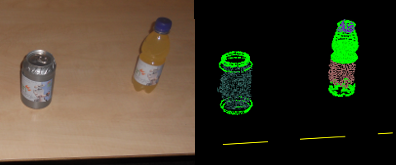
\includegraphics[width=0.5\textwidth]{Images/object_detector.png}}
	\caption{Result of the tabletop object detector. The segmented clusters are coloured and a green wire frame is drawn 
	when an object is recognized.}
	\label{fig:tabletop}
\end{figure}

To detect the tabletop, fast plane detection is used \cite{plane}. The biggest recognized plane will be seen as a 
tabletop, meaning that a wall can also be seen as a 
tabletop if Eva is seeing one.

For more information about the tabletop object detector, please refer to 
\url{http://www.ros.org/wiki/tabletop\_object\_detector} \cite{tabletop}.

The tabletop object detector was used in this project because the results in segmenting and distinguishing the objects 
were better than the package used previously, namely RoboEarth \cite{Roboearth}. Although it was easier to add objects to 
the database of RoboEarth, the detection of objects was not reliable, thus making the tabletop object detector the 
better option. However, since RoboEarth is still a work in progress, it is anticipated that detection in RoboEarth 
happens with more success in the future, so it will be a good alternative if improvements are made.

\subsubsection*{Eva\textquotesingle s arm}
For Eva to successfully manipulate objects, she needs an arm. This arm was designed taking into account a set of 
requirements and constraints. The most important constraint was development time; to allow for some testing time, the 
whole arm would need to be created within a month. To create the arm within a tight budget means reducing the amount of 
expensive components such as motors. Another constraint is the amount of power the arm can consume. As Eva runs on 
batteries, it is important to minimize energy consumption, in order to maximize time between charge.

The goal for the prototype was to pick up small objects weighing up to $2kg$ from a table. Not every table is the same 
height and reaching a kitchen sink is required as well. This means the arm has to reach at least from $0.6m$ to $1.0m$ 
height. When picking up an object from a table, the object will not always be at the edge of the table, so the arm should 
be able to pick up objects that are placed at least $0.30m$ from the edge of the table. Furthermore, to avoid toppling 
and to work efficiently, the weight of the robotic arm should be as low as possible, especially at the end of the arm. 
For aesthetic purposes the arm has to be as compact as possible.

\begin{figure}[h]
	\centering
	\mbox{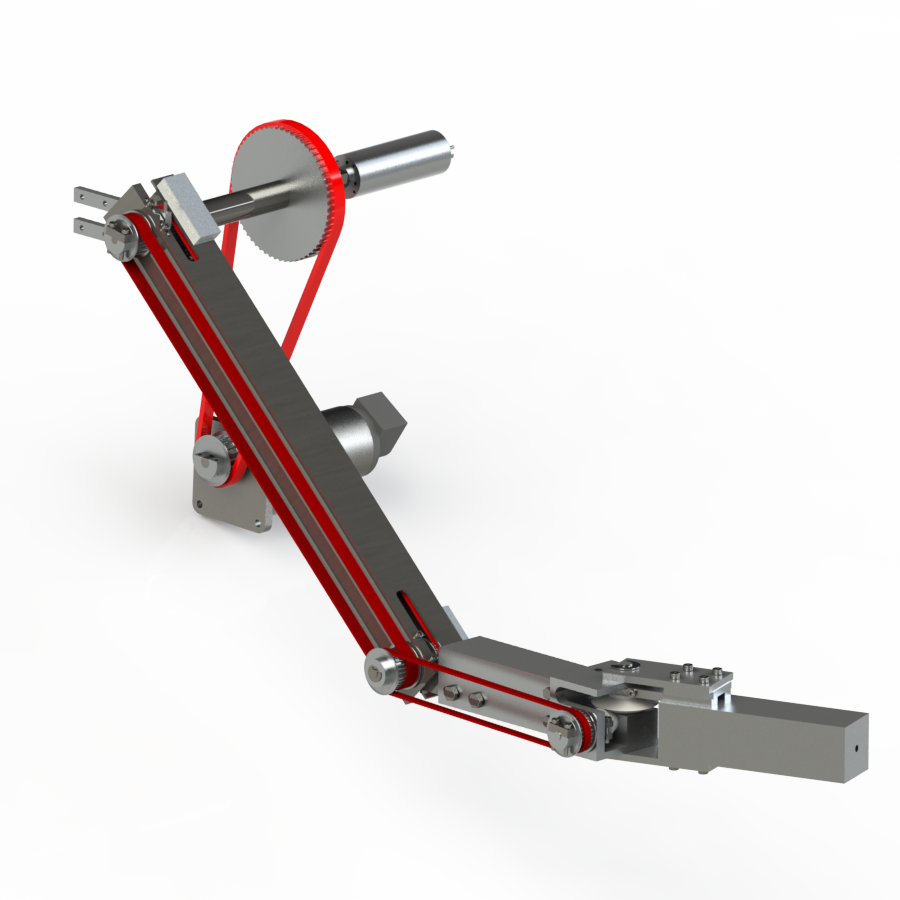
\includegraphics[width=0.5\textwidth]{Images/armMechOverview.png}}
	\caption{Mechanical design of Eva\textquotesingle s arm}
	\label{fig:armMechOverview}
\end{figure}

Summarizing the requirements, the arm should contain as few motors as possible to reduce costs, complexity and power 
usage. If possible, it would be preferable not to place these motors in the arm itself, to keep the arm as lightweight as 
possible. The arm should be able to pick a $2kg$ object from a height between $0.6m$ and $1.0m$. These requirements 
resulted in the arm as designed for Eva, see fig. \ref{fig:armMechOverview}.

The arm can be folded compactly along Eva\textquotesingle s body when not in use, while it can be stretched pretty far 
when grasping an object at table height. The elbow could be driven by a third motor, or kept fixed so the lower arm is 
always horizontal. The last option was chosen, since adding this third motor would make the arm more complex than 
required for the first prototype. The arm can move up and down, move sideways and is connected to the body on a position 
at shoulder hight. This combination gives the arm a humanoid look, but this was not intentional. It is just a result of 
the requirements described earlier.

\subsubsection*{Inverse kinematics}
At first, the Arm navigation stack of ROS was used to position the arm of Eva. However, this stack could not be used in 
the end because it requires an urdf model of the arm \cite{urdf}, which could not be made for Eva\textquotesingle s arm 
(It was not possible to create a link that always stays horizontal). Also, the Arm navigation stack was over complex for 
our purposes, so in the end the inverse kinematics were calculated by ourselves.  

As mentioned in the previous section, Eva\textquotesingle s arm uses two motors to position the gripper: one for moving 
the arm sideways and one for moving the arm in height. In order to position the gripper to a desired position, inverse 
kinematics are used to calculate the joint positions of the motors for a given coordinate in the coordinate frame of the 
arm. On the other hand, forward kinematics are used to calculate the current position of the arm, which is used as 
feedback for positioning the gripper. 

Although this is a deprecated way to position the gripper because of the complexity of inverse kinematics  (Nowadays, 
jacobians \cite{jacobian} [p. 65-69] are used to solve the inverse twist 
problem for the gripper which enables positioning by speed control), in Eva\textquotesingle s case, this problem was 
very easy to solve because her arm only has two degrees of freedom. 

Given the coordinates x and z, the inverse kinematics of the arm are solved by the following formulas. Note that the y 
coordinate of the gripper depends on the z coordinate because the link in the middle always stays horizontal, so it is 
not necessary to take that into the calculations. The first formula calculates the angle for the shoulder, the second 
formula calculates the angle for the ``wrist''. See also \ref{fig:IK0} , \ref{fig:IK2} and \ref{fig:IK1} for drawings 
used for the calculations.

\begin{equation*}
\alpha = \arcsin(z_4/L1)
\end{equation*}

\begin{equation*}
\beta = -1 * \arcsin(x_4/(L3 + L4))
\end{equation*}

Also, the following formulas are used to keep track of the position of the gripper, given an angle $\alpha$ for the 
shoulder and an angle $\beta$ for the ``wrist'' link:

\begin{equation*}
z = \sin(\alpha)*L1
\end{equation*}

\begin{equation*}
x = \sin(-1 * \beta)*(L3 + L4)
\end{equation*}

\begin{figure}[h]
	\centering
	\mbox{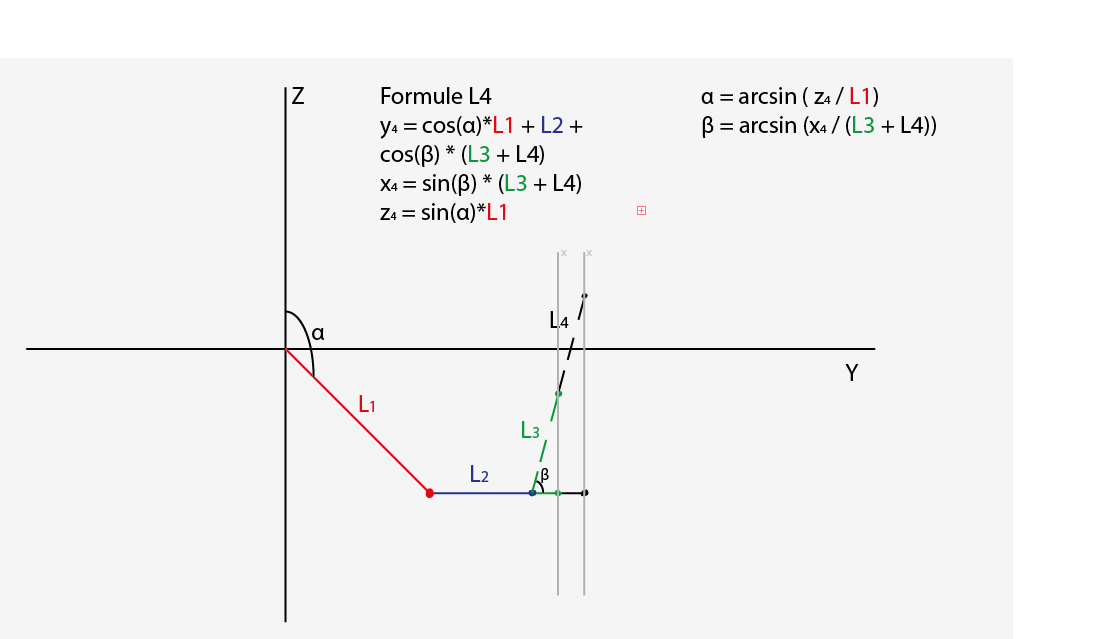
\includegraphics[width=0.5\textwidth]{Images/3d_zijenbovenaanzicht.png}}
	\caption{Side and top view of the arm with calculations of the kinematics.}
	\label{fig:IK0}
\end{figure}

\begin{figure}[h]
	\centering
	\mbox{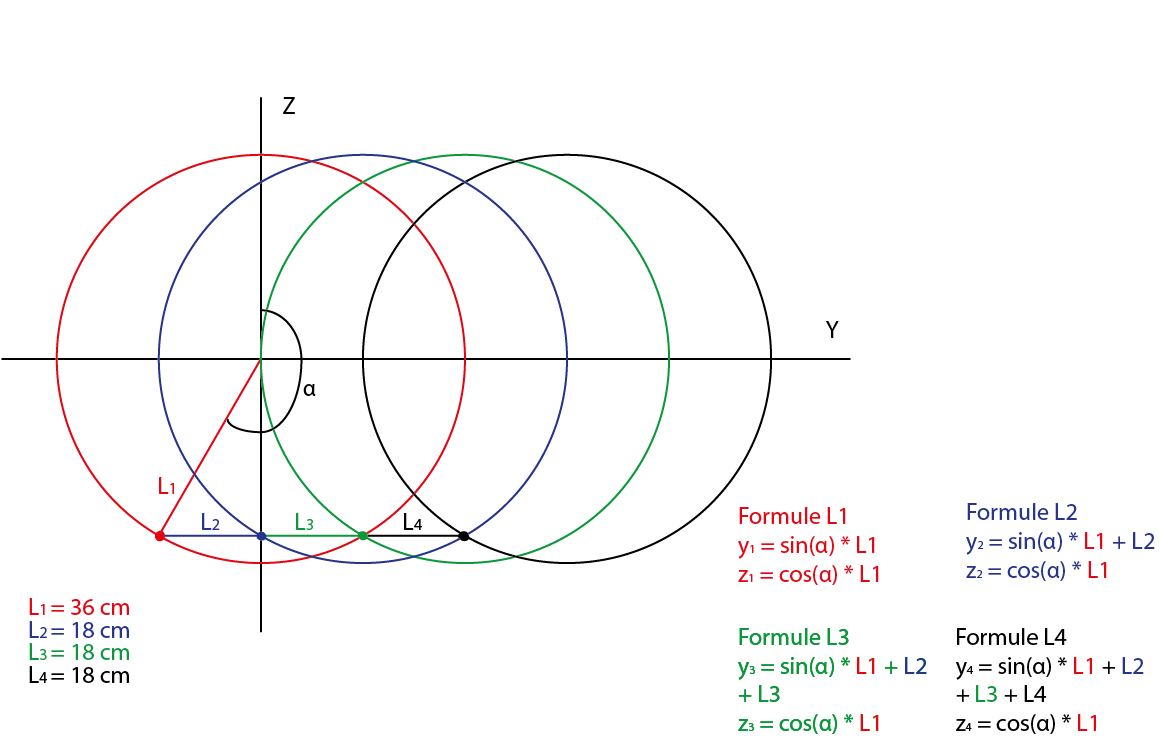
\includegraphics[width=0.5\textwidth]{Images/2d_zijaanzicht.png}}
	\caption{Side view of the arm with calculations of the kinematics.}
	\label{fig:IK2}
\end{figure}

\begin{figure}[h!]
	\centering
	\mbox{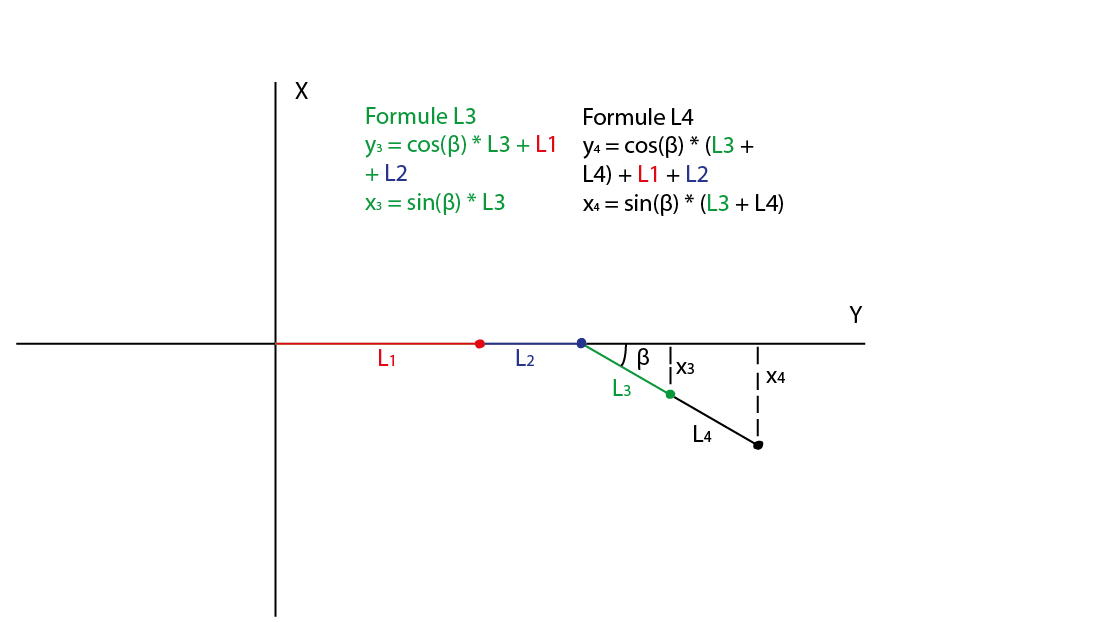
\includegraphics[width=0.5\textwidth]{Images/2d_bovenaanzicht.png}}
	\caption{Top view of the arm with calculations of the kinematics.}
	\label{fig:IK1}
\end{figure}

\subsection*{Navigation}
Navigating Eva in an environment consists of three parts. Firstly, Eva needs to know her surroundings; she needs to map out the environment. Secondly, she needs to plan a path from where she is to where she wants to go. Thirdly she needs to know how to execute this path as good as she can.

\subsubsection*{Object avoidance}
Object avoidance is needed for Eva to keep herself safe, but also to keep the environment safe from her. Eva uses ultrasone 
sensors to detect objects in her environment and scales the speeds of her wheels according to the distance to the 
detected object and the position of this object. Eva has six sensors in front, two in the back and one on each side. The 
sensors in the front are used in units. So if Eva hears an object on the left, she will go right and vice 
versa. In essence, Eva avoids objects as a Braitenberg vehicle \cite{braitenberg} [p. 8]. For more information about object avoidance, see the technical document\cite{Tech} .

\subsubsection*{Map creation}
The GMapping package in ROS was used to create a map of the environment. GMapping \cite{GMapping} is a SLAM algorithm, 
which stands for \textit{Simultaneous Localization And Mapping}. The algorithm takes in laserscan and odometry data and 
this data is converted into a map. There is no laser present on Eva, so this data had to be substituted by Kinect data, 
which is an easy conversion.

At this stage there is a map created by GMapping, but in PGM format (similar to the image bitmap format). Recast 
\footnote{http://code.google.com/p/recastnavigation/} is used to convert a map into a navigation mesh, which is later used to determine a path from point A to point B, however Recast accepts only maps of the format OBJ: a 3D representation 
format \cite{wavefront}. To convert from PGM to OBJ, a custom converter had to be written \cite{Tech} . Recast is then ready to create a navigation mesh on the map. This mesh defines where Eva is allowed to walk, it does so using a set of parameters, of which the most important one is the radius of Eva. With this information, Recast can determine the walkable areas in the map. This mesh can later on be used to determine paths for Eva.

\subsubsection*{Global planner}
Originally the navigation stack in ROS was used as global planner. This navigation stack however proved to be a big black box; if it did not work, it was hard to figure out why. On top of that, it required a lot of processing power. The laptop used in Eva could not handle this navigation quickly enough and was sometimes behind on reality. For these reasons and because of earlier experience with a path planner designed for games (which could be applied here too), it was decided to scratch the ROS navigation stack and create one based on Recast/Detour. The efficiency of this path planner is much better, because most of the calculation is done before navigating and it is optimized to be functional in games with many agents constantly requesting new paths.

\subsubsection*{Planning}
Calculating paths on the generated navigation mesh is done using Detour, which is supplied together with Recast. Detour is handed a starting location (the position of Eva) and a goal location. Using the navigation mesh supplied earlier, a path is calculated (ideally exactly on the goal location, but if this is not on the navigation mesh or unreachable, it gets as close as possible). The path is described by waypoints, where the number of waypoints can be increased, making the path smoother.

\subsubsection*{Executing a path}
Originally Eva would strictly follow this path. What this means is that she would keep rotating until she was facing the 
path, then drive forward until she reached a waypoint and then rotate again until she faced the next waypoint. This looked very unnatural and very static. 

For this reason a new way to execute the path was designed. This enabled Eva to deviate from the path just slightly, enough 
to take corners while still driving forward. The idea behind this new way of executing the path, is that Eva looks a 
certain distance forward on the path and tries to drive to that point. When Eva is nearing a corner, her focus point is 
just a bit beyond this corner, thus she cuts it slightly while still driving forward. To prevent her from flying out of a 
corner, the forward speed is reduced as the angular speed increases. In effect this means that when she is taking corners, 
she slows down and after having taken the corner speeds up again. This path execution can be seen in figure 
\ref{fig:global_path}. The green line is the complete path, whereas the black line points towards the focus point of Eva. 
The longer this line, the faster she drives forward. In simple words this black line can be seen as a spring attached to 
Eva. For this figure, Eva was artificially pushed away to test how well she would return to her path.
\begin{figure}[ht!]
	\centering
	\mbox{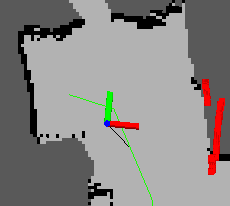
\includegraphics[scale=0.4]{Images/global_path.png}}
	\caption{Eva executes a (global) path.}
	\label{fig:global_path}
\end{figure}


\end{document}